\documentclass[18pt]{article}
\usepackage[utf8]{inputenc}
\usepackage[T1]{fontenc}
\usepackage{ragged2e}
\usepackage{caladea}
\usepackage{graphicx}
\usepackage{longtable}
\usepackage{wrapfig}
\usepackage{rotating}
\usepackage{epigraph}
\usepackage[normalem]{ulem}
\usepackage{hyperref}
\usepackage{amsmath}
\usepackage{amssymb}
\usepackage{capt-of}
\usepackage{hyperref}
\usepackage{fancyhdr}

\title{
 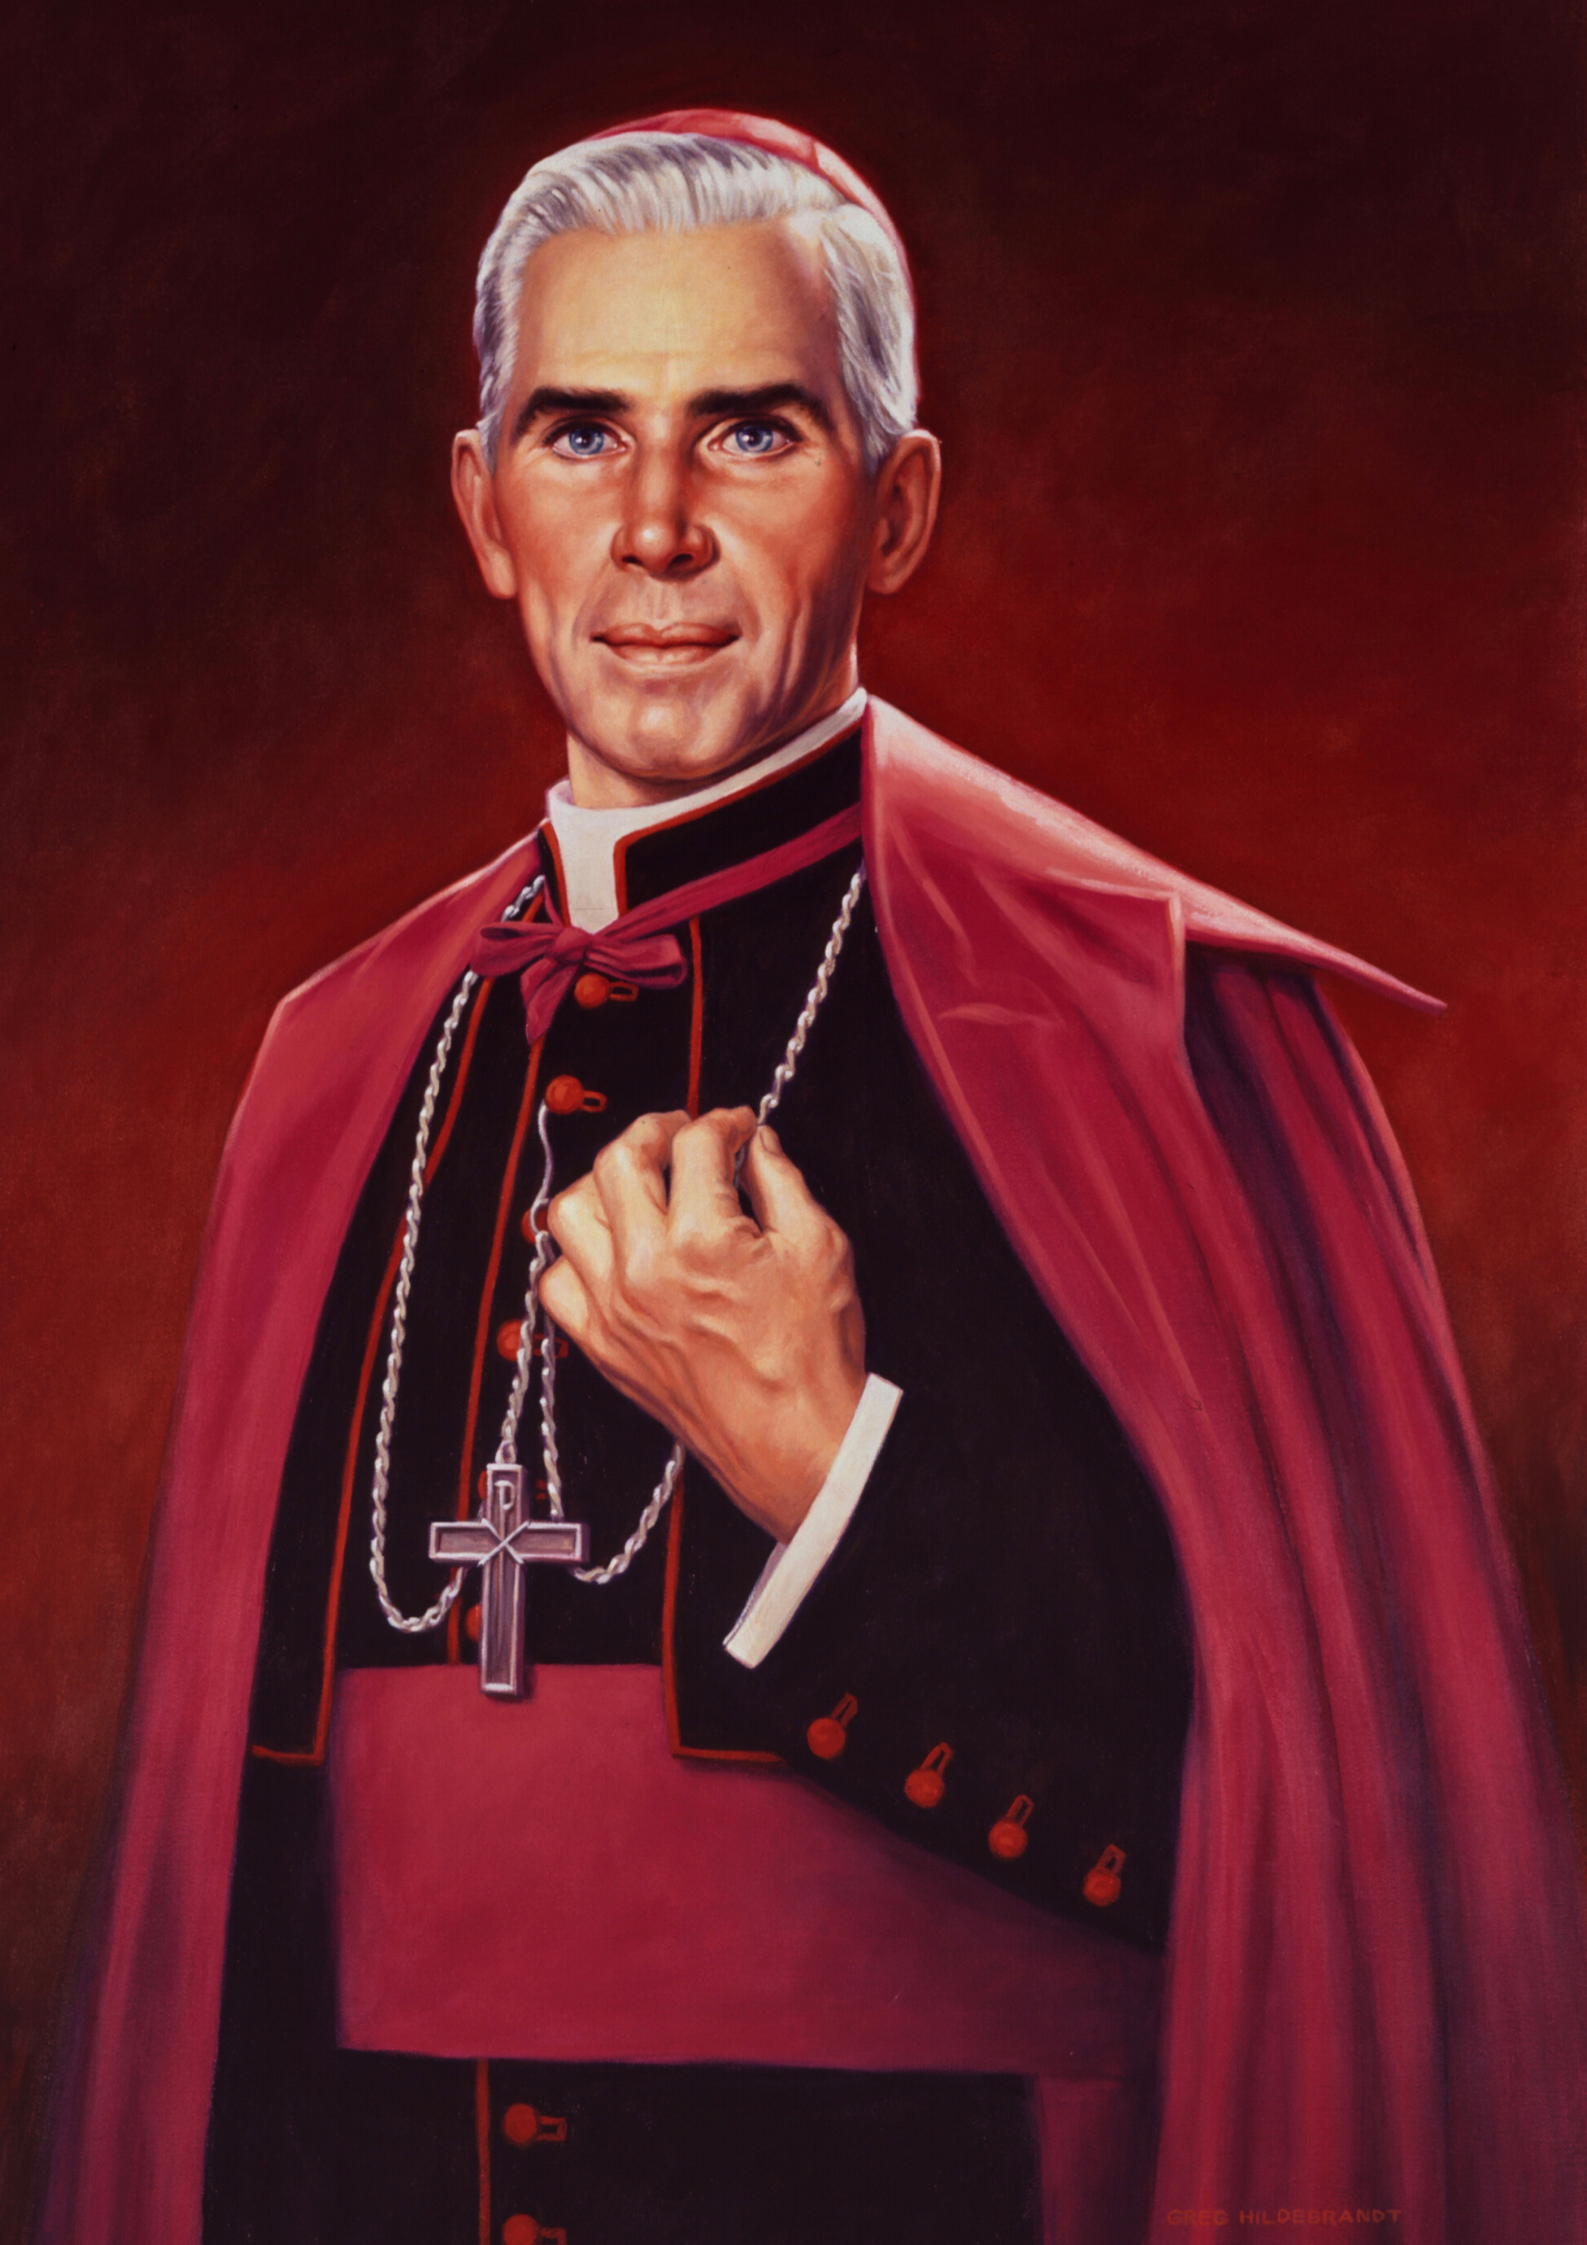
\includegraphics[scale=.24, trim={10cm, 0, 10cm, 0}]{./assets/imagem.jpg}
  \par
   NOVENA a São Rodrigo de Córdoba}
  \date{Início da Novena : 04/03 - Data Litúrgica: 13/03} 
  \author{Garamog, Nina Freitas}


% Comando para fazer "Sumário" não aparecer no Sumário.
\renewcommand{\contentsname}{Sumário}
\begin{document}

\begin{document}
\maketitle
\tableofcontents

\thispagestyle{empty} %zera a primeira página

\pagestyle{fancy}
\fancyhf{} % clear existing header/footer entries
\fancyfoot[LO, CE]{
\includegraphics[scale=0.2]{./assets/cross.png} São Rodrigo de Córdoba, rogai por nós!
}
% Place Page X of Y on the right-hand
% side of the footer
\fancyfoot[R]{\thepage}

\centering
\vfill
Visite-nos no Telegram: \url{https://t.me/CotidieNovena}

%%%%%%%%%%%%%%%%%%%%%%%%%%%%%%%%%%%% História %%%%%%%%%%%%%%%%%%%%%%%%%%%%%%%%%%%%%%%%%%

\begin{justify}
 São Rodrigo (falecido em 857) Sacerdote e mártir de Córdova. Nasceu como Rodrigo no sul de Espanha no século IX e morreu por decapitação em 857 em Córdova, Espanha. Também é conhecido como Rodriguez, Rudericus, Roderic, Ruderic. O Martirológio Romano inclui-o, juntamente com Salomão, sob o nome latino de Rudericus na lista atual.

Rodrigo era um sacerdote de Córdoba, na Andaluzia, região que fazia parte do reino dos visigodos de Espanha.
São Rodrigo por Murillo

Encontrava-se numa situação não rara naquele território, então sob domínio árabe - um dos seus irmãos tinha permanecido cristão e o outro tinha-se tornado muçulmano. E ele, Rodrigo, morreria às mãos dos árabes, pelo que é habitualmente representado com as vestes de sacerdote e com a palma dos mártires.

Mas, neste caso, não se trata da forma habitual de perseguição. Na altura, na região, muçulmanos, cristãos e judeus coexistiam pacificamente. Rodrigo foi vítima de desavenças e violências familiares e fraternas.

O irmão muçulmano censurava o terceiro irmão pela sua “obstinação” em permanecer cristão. Rodrigo tenta fazer as pazes entre os dois, mas sem sucesso.

Um dia, de fato, Rodrigo encontrou os dois numa luta física entre si. Quando tentou dividi-los, como é frequente, os dois viraram-se contra ele e começaram a bater-lhe. Ele caiu inconsciente sob os seus golpes. Nessa altura, o irmão muçulmano levou-o numa carroça - parecia morto - e, perante o espanto do povo, deu uma explicação mentirosa - disse que Rodrigo estava gravemente doente e que, sentindo a morte próxima, também ele se tinha tornado muçulmano.

O boato espalhou-se, mas Rodrigo, quando recuperou, não sabia desta calúnia. Curado, regressou a Córdova com as suas vestes sacerdotais e o seu irmão-acusador arrastou-o até ao juiz muçulmano dizendo: “Este tinha-se tornado um seguidor do Islão e agora regressou ao cristianismo, traiu a nossa fé.” Esta acusação seria considerada como apostasia ao abrigo da lei da Sharia e incorreria na pena de morte!

O juiz tentou ajudar Rodrigo a salvar-se, sugerindo mesmo uma declaração de fidelidade ao Islão, que o libertaria imediatamente, sem lhe pedir compromissos concretos sobre a prática da fé muçulmana. Mas Rodrigo manteve a sua lealdade e recusou-se a negar Cristo e a sua Igreja, preferindo morrer. Presumimos que tenha negado as mentiras contadas pelo irmão, mas não há qualquer relato sobre isso. O juiz, relutante, condenou-o então à morte, por insistência do irmão. Fratricídio, mais do que perseguição.

Rodrigo foi então condenado à morte juntamente com outro cristão chamado Salomão, condenado pelo mesmo motivo. Atirados ao rio Guadalquivir, os corpos foram recuperados pelos cristãos, que sepultaram Rodrigo na Basílica de San Genesio, perto de Córdova, e Salomão na vizinha Igreja dos Santos Cosme e Damião.

Para ambos, a santidade foi proclamada imediatamente, a partir de baixo. A festa é celebrada desde 1581, hoje, 13 de março.

O Convento e Hospital de S. Rodrigo em Cabra, fundado no século XVI, tem o seu nome.


\href{https://anastpaul.com/2021/03/13/saint-of-the-day-13-march-saint-roderick-died-857-priest-and-martyr/}{\textbf{Créditos: } Anast Paul}

\end{justify}

%%%%%%%%%%%%%%%%%%%%%%%%%%%%%%%%%%%%% Orações %%%%%%%%%%%%%%%%%%%%%%%%%%%%%%%%%%%%%%%%%%%
\begin{justify}

\newpage
\begin{center}
 \section{Orações}\label{sec:Orações} % (fold)
\textit{Em nome do Pai, e do Filho, e do Espírito Santo. Amém.}
\end{center}

Ó Glorioso Mártir, São Rodrigo, que mesmo diante do engano e da calúnia, da confusão e da violência, preferistes morrer a renegar a fé em Cristo, intercedei por nós para que nos seja concedida de Deus a graça \textbf{\textit{(faça o pedido)}} que tanto necessitamos. Faz com que, seguindo vosso exemplo, tenhamos coragem de Deixar tudo para viver por Cristo.

\begin{center}
\textbf{\textit{Pai Nosso, Ave Maria e Glória ao Pai.}}
\end{center}

\vfill

\begin{center}
\section*{São Rodrigo, Rogai por nós!}
\end{center}

\vfill


\end{justify}

\end{document}
